\documentclass[a4paper,10pt]{article}
\usepackage{amsmath}
\usepackage{amsfonts}
\usepackage{graphicx}
\usepackage{verbatim}


\title{A Tool to generate unit tests }

\author{UNICA}

\begin{document}
\maketitle



\begin{abstract} 
The agent-based representation of the economic model is made by a lot of functions that we need to be sure that it are working properly. The smallest function for an agent could be considered the transition function, this function allows the agent to act and to communicate with the others agents. The correct operation of all transition functions  is a necessary condition for the correct functioning of the entire system.
The best way to test small parts of the system is the unitary test provided with a tool that collect all units in one o more suits and able to run automatically. We present a tool that provide an automatic way to write and run a collection of suites generating code from a collection of a suites, where each suite is described by a specified markup language.
\end{abstract}
\tableofcontents

\section{Introduction}

\subsection{The unit-test generator tool:basics ideas}

The agent-based representation of the economic model is made by a lot of functions that we need to be sure that it are working properly. The smallest function for an agent could be considered the transition function, this function allows to the agent acting and communicating with the others agents. The correct operation of all transition functions is a necessary condition for the correct functioning of the entire system.
The best way to test small parts of the system is the unitary test provided with a tool that collect all units in one o more suits and able to run automatically. In a system is large it is a good practice to divide the system in modules, which have to be tested with an automatic tool respecting the modular organization. In order to do this specific ... 

%\verbatiminput{rules/grammar_rule.txt}
The rules that is following satisfy the lexical-grammar definition that we have defined before:
\verbatiminput{rules/rules.txt}

\section{General description}
The automatic tool to run unitary test run a collection of suites, 
where each suite contain a collection of unitary tests. 
Each suite is related basically to a module maintaining the preexistent subdivision, but it is possible to build more suites  for a single module, for example we can write three suites for the financial market regarding each agents that act in the financial market, so we will have a better subdivision. The set of the suites is collected in a xml file, this file allows to configure the system and group the suites.   
\begin{figure}
\centering
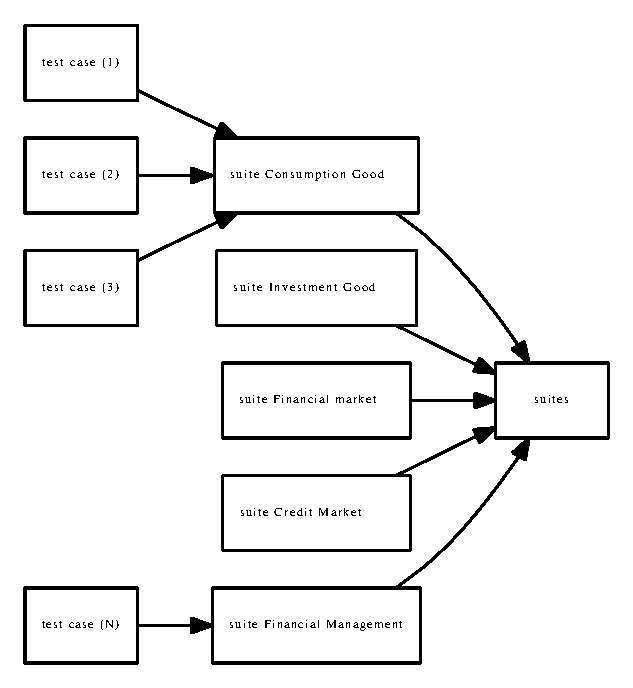
\includegraphics[scale=0.9]{graph/suites} 
\end{figure}
\subsection{The configuration file}
The set of the suites of the entire model are grouped by a configuration file, this file are used to configure the paths of each suite and the path of the model. This file is placed in the top of model in the same folder that contains the model description.
\begin{figure}
\label{fig:fig2}
\verbatiminput{code/suites.xml}
\caption{the configuration file suites.xml}
\end{figure} 
The previous code describes the configuration of the testing for the eurace model, it contains two fondamental tags that are following:
\begin{itemize}
\item the tag \textbf{modelPath}, associate the system of test to the FLAME agent model;
\item the tag \textbf{suitePath}, it allows to add a new suite associating its path.
\end{itemize}
\subsection{The suite}
The suite is described by a file, this file has the extension .xml and  has to be placed in the linked module, in the same folder of the associated sub-module. The suite is identified by a name and is characterized by a collection of unitary tests. The agent model is set with a list of constants that need to be specified.
The composition and elements of a suite is opened with the tag called \textbf{suite} and its specification is characterized by the following tags:

\begin{itemize}
\item the tag \textbf{name}: this tag specified the suite name, this name must be unique in the system.
\item the tag \textbf{constants},this tag contain the values of each costants. We must specify only the constanst that are used in the collection of test-cases, this definition is explained with more details in the next paragraph.
\item the tag \textbf{unittest}: this tag open the unit-test specification and it could be repeated more times , each time that we have to define a test-case.
\end{itemize}
\subsection{The unit test}
The  unit test is set by the following items:
\begin{itemize}
\item the \textbf{name of the test}. This name has to be unique in the  system.
\item the \textbf{name of the transition function} that will has to be tested.
\item the name of the owner of the transition function. This part specifies the type of agent (for example Household or Firm) that are subject to the test.
\item the \textbf{declarative part}. This part is important because it specifies how the assertion parts have to be built .
\item the \textbf{fixture}. 
\item the \textbf{expected values}.
\end{itemize}
\subsubsection{The declarative part}
The declarative part specifies the variables and messages that are subject to assertions. This part is opened with the tag called \textit{declaration} and contains a list of variables and a list of messages. The list of variables 
The following code shows an example of a typical declarative part:
\verbatiminput{code/declarative.xml}
The xml code above shows two variables and a messages that are subject to assertion. The \textbf{test\_generator} tool generate three types of assertion: the first assertion is related to the \textit{assetsowned}, the second to \textit{pending\_orders } and finally the third is related to the \textit{order }message.
\subsubsection{The fixture}
The fixture is a set of memory variables and input messages, initialized to proper values, used
as repeatable input data for the tests. Each time a test case is run, its fixture is
reinitialized, because previous tests might have corrupted the fixture, making
the test fail not due to errors in the code, but to wrong test data. By defining
a fixture, you decide what you will and won't test for. A complete set of tests
for a transition function  will have many fixtures, each of which will be used by many tests,
in many ways.
This part is opened with the tag called \textbf{fixture} and contains a  list of the initialization values of agent's variables and a list of the initialization values of messages.
The following code shows an example of a typical fixture part:
\verbatiminput{code/fixture.xml}
\subsubsection{The expected values}
A Test Case stimulates a Fixture and checks for expected
results. If the tests are unsuccessful, they have to provide helpful information
about the kind of error and about his location, the system that launch the test shows a summary of all test belonging from all suite. To this purpose,
the framework is endowed with standard checking functions (Checks)
able to test Boolean conditions and to report automatically the results
and the system state in the case of failure. 
The checks need an expected state of the agent and the expected output messages. The expected values part is opened with the tag called \textbf{expected\_states} and contains a  list of the expected values of agent's variables and a list of the expected values of output messages.
The following code shows an example of a typical fixture part: 
\verbatiminput{code/expected.xml}
The xml code above shows two agent's variables that are the expected state of the Household. The expected\_state parts don't contain a list of expected messages because the related transition function don't involve any output message.

\section{Quick start guide}
Here is a set of steps for setting up and generate C code of unit test and run the test automatically . Details and instructions for
a more thorough tour of \textbf{test\_generator}  features, including installing, validating,
and using the performance evaluation tools, are given in the following sections. 

\subsection{Downloading}
The first step is to download the test\_generator and install any necessary files. 
It needs the  libxml and CUnit library that have to be installed properly.
The  way to get test\_generator is to use the repository at the address  http://ccpforge.cse.rl.ac.uk/svn/eurace/tests. 
Get the the entire folder unit-test-generator that contain the following files:
main\_code.c, Makekile , datatype.c.tmp , header.h.tmp , Suite.h.tmp,
Suite.c.tmp, messages.c.tmp, LauncherTest.c.tmp
Now you are ready to build.
\subsection{Making}
Before you can use \textbf{test\_generator}, you must make it. \\
Make test\_generator\\
\% make \\
This may take a while, depending on the load on your system and on your file server,
it may take anywhere from a few seconds to an minut or more.
\subsection{Generating test case and suite organization}
The test\_generator generate code by using the model information an the information contained in the files called suite.xml and present in each module. 
The code generated is compounded by some C code files and a Makefile called Makefiletest, 
\subsection{Running}
Run a simple integrity test:\\
\% cd ../integrity\_tests\\
\% ./integrity tests/rules.xml target.txt\\
At this point you have run an integrity test on your system. 
\subsection{The examples: rules.xml}
The Integrity distribution contains a simple programs, which are located in the
integrity source tree.
The rules.xml \ref{fig:fig1} is a simple example which is explained how configure an integrity test.
\begin{figure}
\label{fig:fig1}
\verbatiminput{../tests/rules.xml}

\caption{the configuration file rules.xml}
\end{figure}

\end{document}
